\documentclass[portrait,fontscale=0.35,paperwidth=800mm, paperheight=1200mm]{baposter}


\usepackage[utf8]{inputenc}

\usepackage{calc}
\usepackage{graphicx}
\usepackage{amsmath}
\usepackage{amssymb}
\usepackage{relsize}
\usepackage{multirow}
\usepackage{rotating}
\usepackage{bm}
\usepackage{enumitem}
\usepackage{url}
\usepackage{booktabs}
\usepackage[font=scriptsize]{caption}
\usepackage{framed}
\usepackage{graphicx}
\usepackage{multicol}
\usepackage{txfonts}

\renewcommand{\rmdefault}{phv} % Arial
\renewcommand{\sfdefault}{phv} % Arial
\usepackage[italian]{babel}

%
% Command definitions
%
\newcommand{\problemdomain}{\Omega}
\newcommand{\primalgrid}{\mathcal{G}}
\newcommand{\dualgrid}{\mathcal{\tilde{G}}}
\newcommand{\positionvec}{\bm{r}}
\newcommand{\normal}{\field{n}}
\newcommand{\field}[1]{\bm{#1}}
\newcommand{\fieldfunc}[1]{\field{#1}(\positionvec)}
\newcommand{\tensor}[1]{\field{#1}}
\newcommand{\tensorfunc}[1]{\tensor{#1}(\positionvec)}
\newcommand{\rot}{\nabla\times}
\newcommand{\faradayneumann}{\rot\fieldfunc{e} = -i\omega\fieldfunc{b}}
\newcommand{\amperemaxwell}{\rot\fieldfunc{h} = i\omega\fieldfunc{d} + \fieldfunc{j}_s}
\newcommand{\primaledge}{e}
\newcommand{\primalface}{f}
\newcommand{\dualedge}{\tilde{e}}
\newcommand{\dualface}{\tilde{f}}
\newcommand{\borderprimaledge}{e^b}
\newcommand{\borderdualedge}{\tilde{e}^b}
\newcommand{\primalcurl}{\mathbf{C}}
\newcommand{\dualcurl}{\mathbf{C}^T}
\newcommand{\numatrix}{\mathbf{M}_{\nu}}
\newcommand{\epsmatrix}{\mathbf{M}_{\epsilon}}
\newcommand{\ximatrix}{\mathbf{M}_{\xi}}
\newcommand{\mumatrix}{\mathbf{M}_{\mu}}
\newcommand{\ymatrix}{\mathbf{M}_{Y}}
\newcommand{\mmf}{\mathbf{F}}
\newcommand{\emf}{\mathbf{U}}
\newcommand{\magflux}{\mathbf{\Phi}}
\newcommand{\elecflux}{\mathbf{\Psi}}
\newcommand{\bordermmf}{{\mmf^b}}
\newcommand{\borderemf}{{\emf}}
\newcommand{\basepropagation}{(\dualcurl\numatrix\primalcurl - \omega^2\epsmatrix)\emf}
\newcommand{\basepropagationcompl}{(\dualcurl\ximatrix\primalcurl - \omega^2\mumatrix)\mmf}
\newcommand{\admittancecontrib}{i\omega\ymatrix\emf}
\newcommand{\scatteringborder}{{\partial_s}}
\newcommand{\port}{\Sigma}
\newcommand{\YCalculationPlane}{\Pi}


% Note command:
%  parameter 1: author
%  parameter 2: note text
%\newcommand{\note}[2]{
%    \begin{center}
%        \centering
%        \fcolorbox{red}{YellowGreen}{
%            \mbox{
%                \parbox{0.8\linewidth}{
%                    \begin{center}
%                        \leftpointright~~\textbf{NOTE}
%                    \end{center}
%                    {\footnotesize
%                        \textcolor{red}{\emph{Author:}} #1\\
%                    #2
%                    }
%                }
%            }
%        }
%    \end{center}
%}

% Correction command:
%  parameter 1: author
%  parameter 2: subject
%  parameter 3: status
\newcommand{\correction}[3]{
    \begin{center}
        \centering
        \fcolorbox{red}{GreenYellow}{
            \mbox{
                \parbox{0.8\linewidth}{
                    \begin{center}
                        \smallpencil~~\textbf{CORRECTION}
                    \end{center}
                    {\footnotesize
                        \textcolor{red}{\emph{Proposed by:}} #1\\
                        \textcolor{red}{\emph{Subject:}} #2\\
                        \textcolor{red}{\emph{Status:}} #3\\
                    }
                }
            }
        }
    \end{center}
}



 \newcommand{\compresslist}{%
 \setlength{\itemsep}{1pt}%
 \setlength{\parskip}{0pt}%
 \setlength{\parsep}{0pt}%
 }

\usepackage{tikz}
\newcommand*{\BottomLeftX}{1.0in+\hoffset+\oddsidemargin}%
\newcommand*{\BottomLeftY}{\paperheight-1.0in-\voffset-\topmargin-\headheight-\headsep-\textheight}%
\newcommand*{\AbsolutePosition}[5][]{%
    % #1 = tikz options
    % #2 = x (from south west corner of page
    % #3 = y
    % #4 = text
    \begin{tikzpicture}[remember picture,overlay, ultra thick]
        %\draw [shift={(#2,#3)},#1]  (current page.south west) circle (2pt) 
        \draw [#1]  ($(current page.south west) + (\BottomLeftX,\BottomLeftY) + (#2,#3)$) rectangle ($(current page.south west) + (\BottomLeftX,\BottomLeftY) + (#2,#3) + (#4, #5)$); 
    \end{tikzpicture}%
}

\begin{document}

\definecolor{lightorange}{rgb}{0.9,0.4,0}
\definecolor{lightestorange}{rgb}{1,0.8,0.5}
\definecolor{darkorange}{rgb}{0.2,0.1,0}

\definecolor{uniud-brown}{rgb}{0.239, 0.165, 0.157}
\definecolor{uniud-orange}{rgb}{1.0, 0.4, 0}
\definecolor{uniud-blue}{rgb}{0.467, 0.604, 0.671}

\begin{poster}{
 columns=2,
 % Show grid to help with alignment
 grid=false,
 % Column spacing
 colspacing=0.7em,
 % Color style
 headerColorOne=white,
 borderColor=white,
 % Format of textbox
 %textborder=faded,
 % Format of text header
 headerborder=open,
 headershape=roundedright,
 headershade=plain,
 background=none,
 bgColorOne=cyan!10!white,
 headerheight=0.12\textheight}
 % Eye Catcher
 {
 }
 % Title
 {\Huge Formulazione geometrica discreta per la modellazione\\ nel dominio della frequenza di siti EMC}
 % Authors
 {%\large Dottorando: Matteo Cicuttin - Supervisori: prof. Ruben Specogna, prof. Francesco Trevisan
 }
 % University logo
 {
  %\begin{tabular}{r}
  %  
\includegraphics[width=0.1\textwidth]{img/logo.pdf}\\
    %\raisebox{0em}[0em][0em]{
\includegraphics[height=0.03\textheight]{img/logo.pdf}}
  %\end{tabular}
 }

%%%%%%%%%
\headerbox{\textbf{Introduzione}}{name=intro,column=0,row=0}{
    La simulazione di camere anecoiche rappresenta un importante ambito di ricerca, in quanto permette di avere dati essenziali sulle prestazioni di un sito EMC. Tuttavia la natura matematica del problema e il range di frequenze in gioco pongono ostacoli significativi a tali simulazioni. Essendo necessario l'uso di risolutori diretti, all'aumentare delle dimensioni del sito, dei dettagli geometrici e della frequenza di lavoro la richiesta di risorse di calcolo diventa in breve tempo ingestibile. Al fine di mitigare queste difficoltà sono stati studiati dei modelli equivalenti utili a ridurre in modo drastico il numero di elementi, e dunque di incognite, necessari a rappresentare siti ed oggetti reali. Tali modelli equivalenti riguardano in particolare le pareti anecoiche e le antenne. Le tecniche sviluppate sono state integrate in un simulatore elettromagnetico, appositamente scritto, basato sull'approccio geometrico discreto (DGA).
}

%%%%%%%%%
%\headerbox{\textbf{Formulazione geometrica discreta}}{name=dga,column=0,row=1, below=intro}{
%    Nella formulazione geometrica discreta dell'elettromagnetismo (DGA) il dominio di calcolo $\problemdomain$ è discretizzato in due griglie tetraedriche $\primalgrid$ e $\dualgrid$. $\dualgrid$ è indotta da $\primalgrid$ attraverso la suddivisione baricentrica.
%    Le quantità elettromagnetiche sono associate agli elementi delle due griglie, in particolare:
%    \begin{itemize}
%       \compresslist
%    \item le forze elettromotrici $U_i = \int_{\primaledge_i}\field{e} \cdot d\bm{l}$ sui lati primali $\primaledge_i \in \primalgrid$ e raccolte nell'array $\emf$,
%    \item i flussi magnetici $\Phi_{i} = \int_{\primalface_i}\field{b} \cdot d\bm{s}$ sulle facce primali $\primalface_i \in \primalgrid$ e raccolti nell'array $\mathbf{\Phi}$,
%    \item le forze elettromotrici $F_i = \int_{\dualedge_i}\field{h} \cdot d\bm{l}$ sui lati duali $\dualedge_i \in \dualgrid$ e raccolte nell'array $\mmf$,
%    \item i flussi elettrici $\Psi_{i} = \int_{\dualface_i}\field{d} \cdot d\bm{s}$ sulle facce duali $\dualface_i \in \dualgrid$ e raccolti nell'array $\mathbf{\Psi}$.
%    \end{itemize}
%    Il problema che è necessario risolvere è 
%    \begin{equation}
%    \basepropagation + i\omega\ymatrix = -2i\omega\bordermmf \label{eqn:propagation-DGA},
%    \end{equation}
%    nella quale la matrice $\mathbf{C}$ è l'adiacenza facce-lati, mentre le matrici $\epsmatrix$, $\numatrix$ e $\ymatrix$ sono le matrici dei parametri materiali.
%}
%
%%%%%%%%%
\headerbox{\textbf{Modelli equivalenti di pareti anecoiche}}{name=pbc,column=0,row=2,below=intro}{
L'ottenimento di un modello equivalente di una parete anecoica prevede alcuni passaggi:
\begin{itemize}
    \compresslist
    \item studio di una cella unitaria, svolto forzando un'onda piana di valore noto sulla superfice $\port$ (Fig. \ref{fig:unitcell-sec}),
    \item calcolo dell'impedenza d'onda $Z_{\YCalculationPlane}$ sul piano $\YCalculationPlane$,
    \item sostituzione della cella unitaria con un dominio di sola aria e terminato da un'impedenza $Z_{\YCalculationPlane'}$ su $\YCalculationPlane'$ opportunamente calcolata (Fig. \ref{fig:unitcell-sec-equiv}).
\end{itemize}

        \begin{minipage}{\textwidth}
            \hfill
            \begin{minipage}[b]{0.40\textwidth}
            \begin{center}
                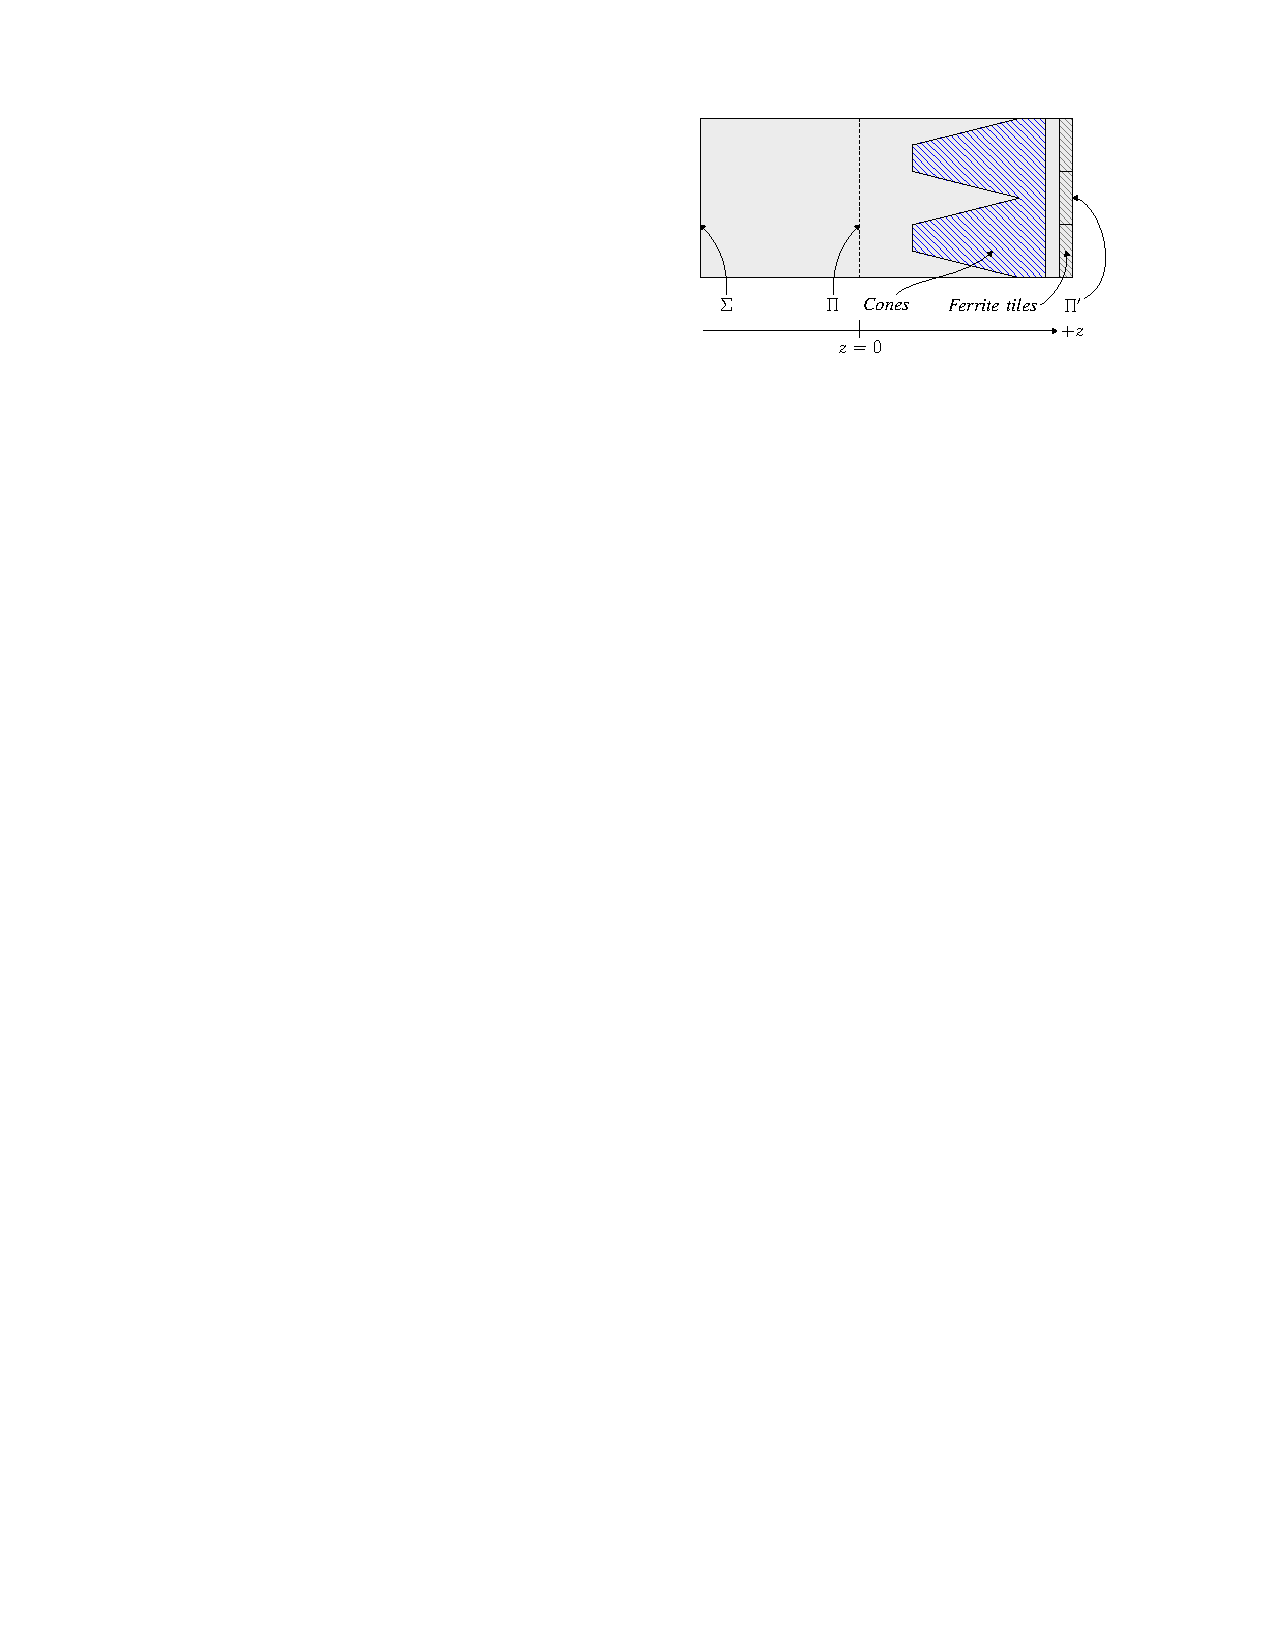
\includegraphics[width=\textwidth]{img/cell_section_poster.pdf}
                \captionof{figure}{Vista in sezione della cella unitaria.}
                \label{fig:unitcell-sec}
            \end{center}
            \end{minipage}
            \hfill
            \begin{minipage}[b]{0.41\textwidth}
                \begin{center}
                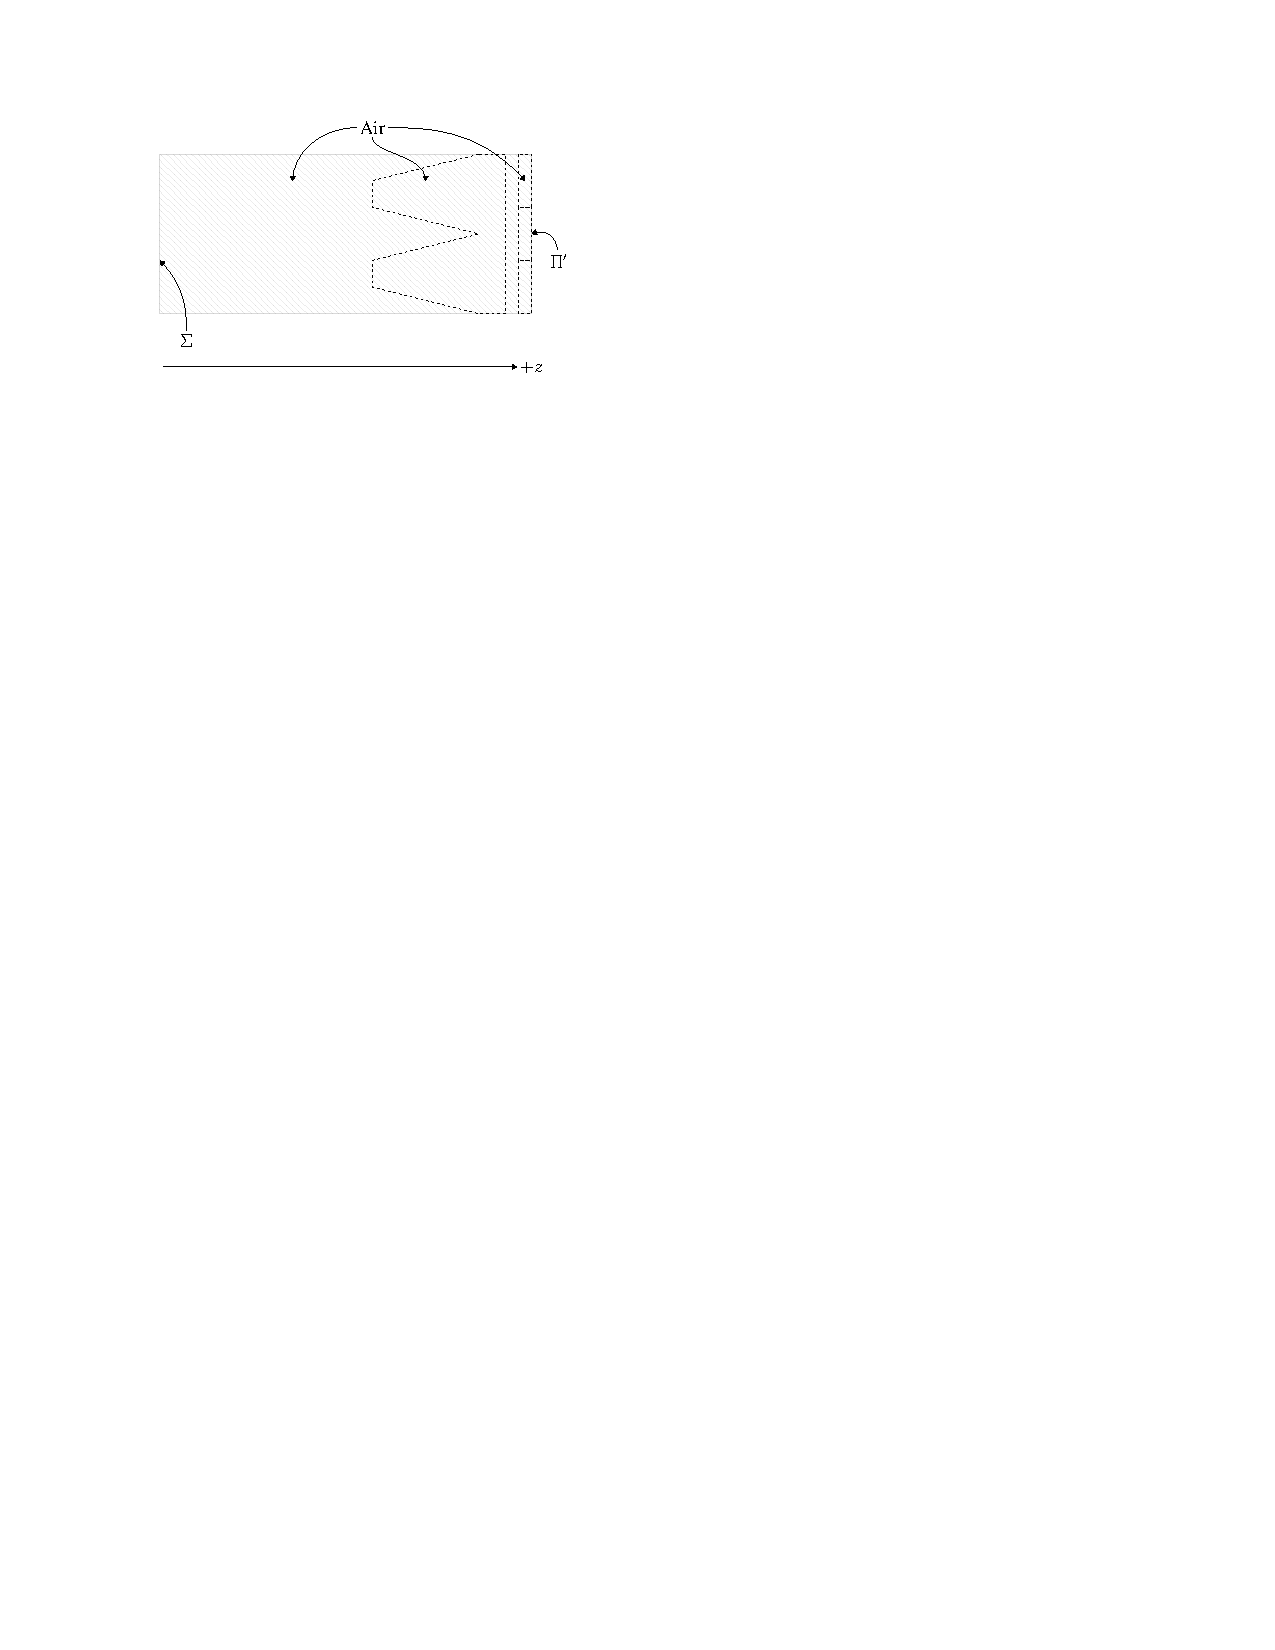
\includegraphics[width=\textwidth]{img/cell_section_equiv_poster.pdf}
                \captionof{figure}{Sezione del modello equivalente.}
                \label{fig:unitcell-sec-equiv}
            \end{center}
            \end{minipage}
            \hfill
        \end{minipage}
        
        \vspace{3mm}

        La simulazione tramite modello equivalente consente una riduzione notevole (20 volte) del numero di elementi necessari a rappresentare una parete, commettendo errori molto bassi nelle zone di interesse.

        \vspace{5mm}

        \hfill
        \begin{minipage}[t]{0.40\textwidth}
           \begin{center}
               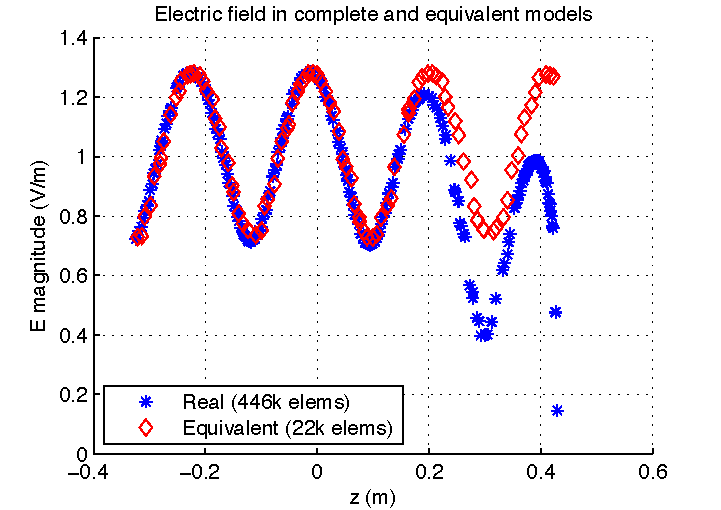
\includegraphics[width=0.8\textwidth]{img/efield_cmp_3.pdf}
               \captionof{figure}{Confronto tra il campo elettrico dato dal modello completo e quello dato dal modello equivalente.}
           \end{center}
       \end{minipage}
       \hfill
       \begin{minipage}[t]{0.40\textwidth}
            \begin{center}
               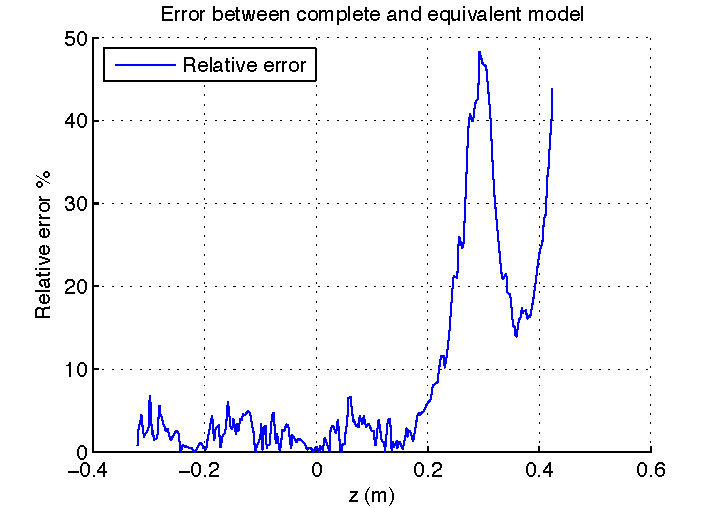
\includegraphics[width=0.8\textwidth]{img/error_3.pdf}
               \captionof{figure}{Errore relativo percentuale del campo calcolato.}
           \end{center}
       \end{minipage}
       \hfill

       % Il campo calcolato tramite il modello equivalente presenta, nella zona di interesse, errori relativi inferiori al 5\%. I tempi di calcolo sono ridotti di circa 60 volte.
}



%%%%%%%%%
\headerbox{\textbf{Elementi radianti equivalenti}}{name=radiators,column=0,row=3, below=pbc}{
    Le antenne sono modellate come sfere sulle quale è proiettato il campo ottenuto tramite altri metodi, ad esempio utilizzando NEC:
    \begin{itemize}
        \compresslist
        \item Non serve tenere in considerazione i dettagli geometrici dell'antenna,
        \item Separazione Total field/Scattered field permette di valutare la reazione dell'ambiente ad una sollecitazione.
    \end{itemize}
}

%%%%%%%%%
\headerbox{\textbf{Validazione della tecnica}}{name=validation, column=1, row=0}{
    La tecnica è stata validata confrontandola con numerosi esperimenti svolti presso il laboratorio di compatibilità elettromagnetica \emph{Emilab SRL}. Tra i più significativi:

    \vspace{3mm}
{\textbf{Esperimento 1}}

    \begin{center}
        \begin{minipage}{0.32\textwidth}
            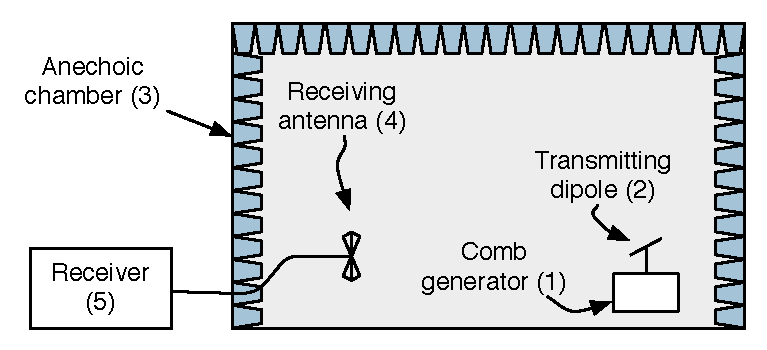
\includegraphics[width=\textwidth]{img/setup}
            \captionof{figure}{Setup di misura}
        \end{minipage}
        \begin{minipage}{0.32\textwidth}
            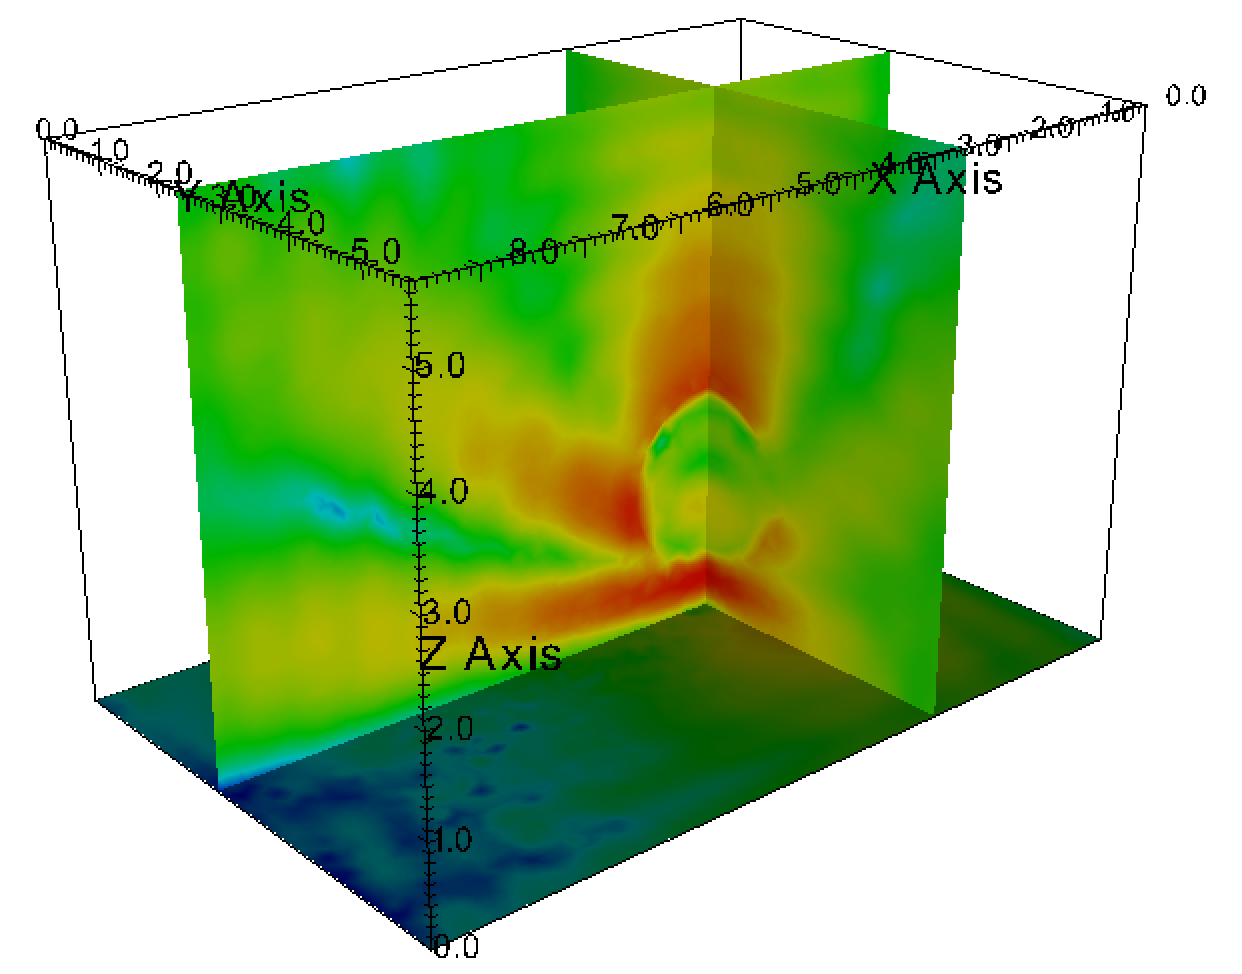
\includegraphics[width=\textwidth]{img/ant230}
            \captionof{figure}{Campo simulato}
        \end{minipage}
        \begin{minipage}{0.32\textwidth}
            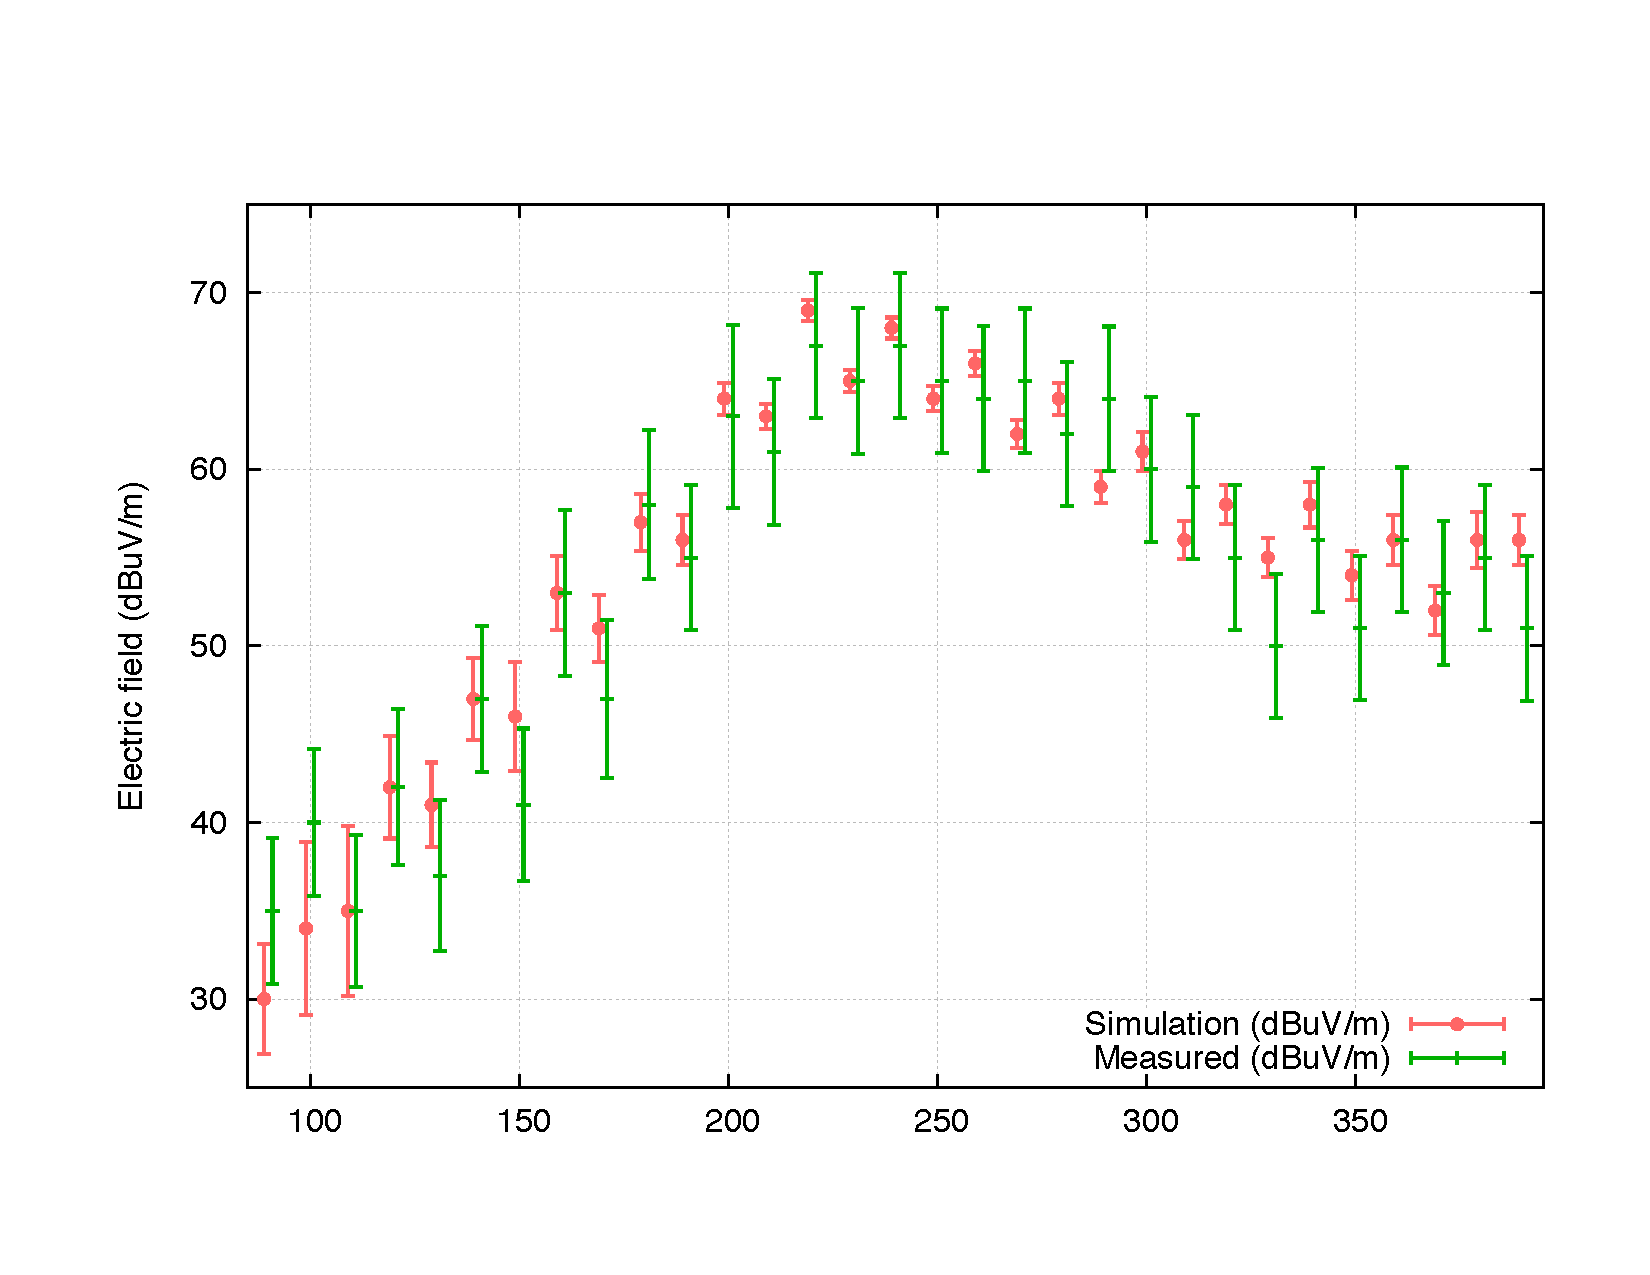
\includegraphics[width=\textwidth]{img/comparison150v}%
            \captionof{figure}{Confronto tra misure e simulazioni}
        \end{minipage}
        \end{center}
        \vspace{3mm}
Un comb generator (1) connesso ad un dipolo (2) irradiava all'interno della camera anecoica (3). Un'antenna biconica (4) posta a 3 metri di distanza e connessa ad un ricevitore EMC (5) permetteva la lettura dei valori di campo elettrico. Le misure sono state eseguite in svariate configurazioni, ottenendo un totale di 558 punti di confronto con le simulazioni.
%I risultati ottenuti sono stati estremamente incoraggianti:
%In Figura 2 a sinistra è rappresentato il campo all’interno della camera in presenza di un dipolo in posizione orizzontale modellato come sfera, mentre a destra vi è il confronto tra i risultati delle simulazioni e le misure reali.

\vspace{3mm}
{\textbf{Esperimento 2}}

    \hfill
    \begin{minipage}[b]{0.48\textwidth}
        \begin{center}
            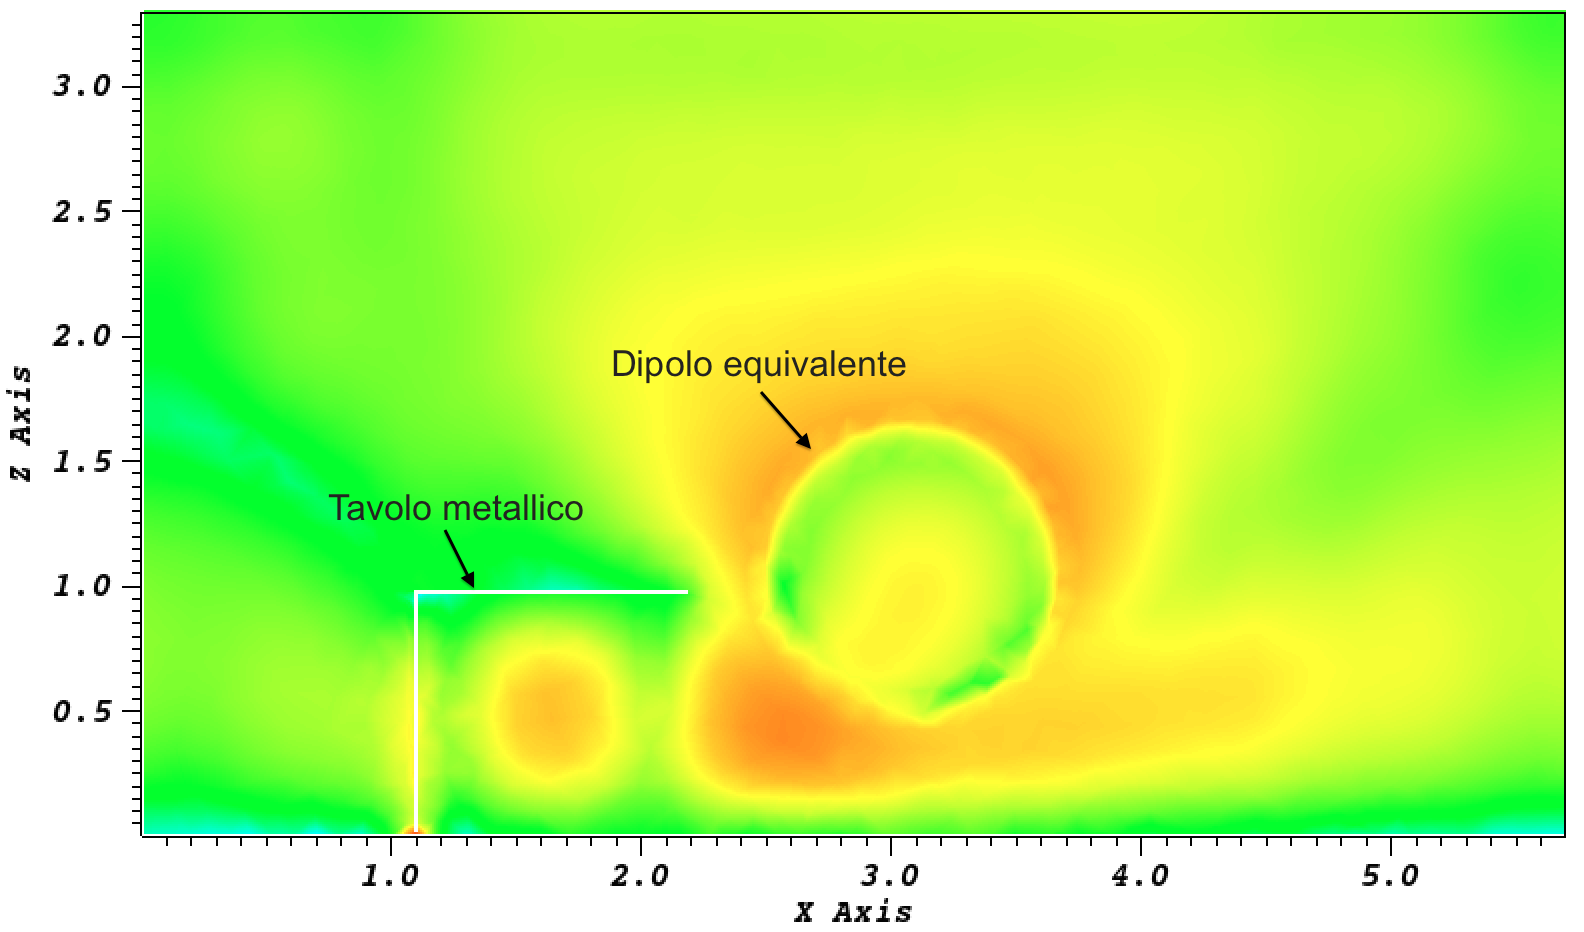
\includegraphics[width=0.8\textwidth]{img/camera.png}%
            \captionof{figure}{Campo simulato}
        \end{center}
    \end{minipage}
    \hfill
    \begin{minipage}[b]{0.48\textwidth}
        \begin{center}
            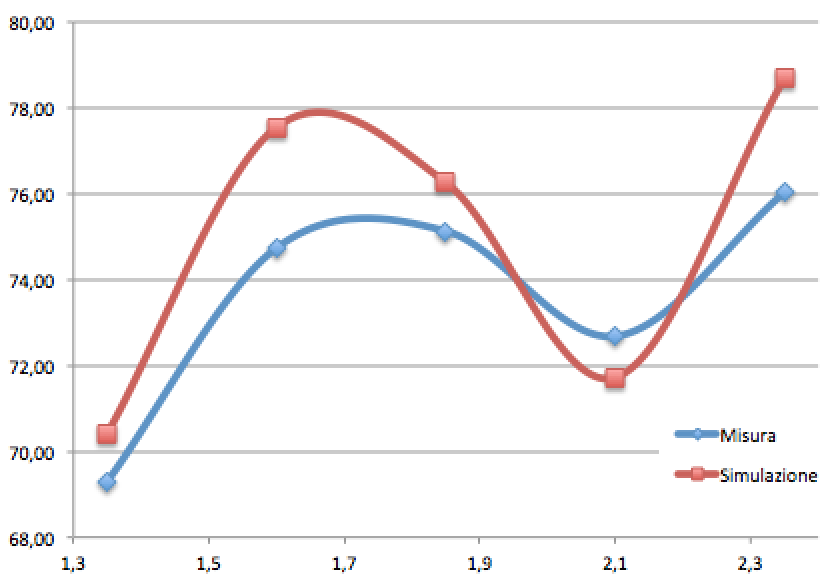
\includegraphics[width=0.6\textwidth]{img/campo}%
            \captionof{figure}{Confronto tra misure e simulazioni}
        \end{center}
    \end{minipage}
    \hfill
    \vspace{3mm}

L'esperimento è stato eseguito in una camera anecoica al cui interno era presente un tavolo conforme a quanto previsto dalle norme relative alle prove in ambito automotive. Ponendo un dipolo equivalente in posizione orizzontale di fronte al tavolo, il simulatore prevedeva la formazione di un'onda stazionaria al di sotto del tavolo stesso. Dalle misure si è riscontrata la presenza di tale onda stazionaria, con valori del tutto simili a quelli previsti dalla simulazione.

    \vspace{3mm}
{\textbf{Considerazioni}}

La moltitudine di confronti effettuati ha confermato la bontà del codice di simulazione
\begin{itemize}
        \compresslist
    \item dal punto di vista predittivo: le configurazioni di campo calcolate rispecchiano quelle misurate nella realtà,
    \item dal punto di vista della validazione delle misure: in svariate occasioni i risultati della simulazione hanno permesso di scoprire errori nella procedura di misura.
\end{itemize}
    
}




%%%%%%%%%
%\headerbox{\textbf{Ulteriori funzionalità}}{name=more, column=1, row=1, below=validation}{
%    \textbf{Perfectly Matched Layers}
%
%    \textbf{Refinement adattativo}
%
%    \textbf{Accoppiamento campi/circuiti}
%}

\headerbox{\textbf{Il codice numerico}}{name=thecode, column=1, row=2, below=validation}{
    Le tecniche sviluppate sono state implementate in un codice DGA scritto appositamente.
    \begin{itemize}
        \compresslist
        \item Multipiattaforma e moderno: scritto in C++14, gira su Windows, Linux e Mac,
        \item Veloce ed efficiente,
        \item Si tratta di un codice generale per la DGA: oltre al modulo per la propagazione ha moduli per conduzione stazionaria, elettrostatica, magnetostatica.
    \end{itemize}
}


%%%%%%%%%
\headerbox{}{name=contacts, column=0, row=4, below=radiators, span=2}{
    \hfill
    \begin{minipage}[t]{0.2\textwidth}
        \textbf{dott. Matteo Cicuttin}\\
        \textbf{Prof. Ruben Specogna}\\
        \textbf{Prof. Francesco Trevisan}\\

        \textbf{Info:}\\
        matteo.cicuttin@uniud.it
    \end{minipage}
    \hfill
    \begin{minipage}[t]{0.4\textwidth}
        \textbf{Riferimenti bibliografici}\\
        {\small
        [1]	S. Chialina, M. Cicuttin, L. Codecasa, R. Specogna, and F. Trevisan, ``Plane Wave Excitation for Frequency Domain Electromagnetic Problems by Means of Impedance Boundary Condition'', IEEE Trans. Magn., vol. 51, no. 3, pp. 1–4, 2015.

        [2] M. Cicuttin, L. Codecasa, R. Specogna, and F. Trevisan, ``Complementary discrete geometric h-field formulation for wave propagation problems'', Proceedings of COMPUMAG2015 conference.
    }
        %\vfill
    \end{minipage}
    \hfill
    \begin{minipage}[t]{0.3\textwidth}
        \textbf{Ringraziamenti}
        \begin{itemize}
            \item Emilab SRL, Amaro (UD) - Laboratorio di compatibilità elettromagnetica
            \item Progetto regionale EMCY
        \end{itemize}
        %\vfill
    \end{minipage}
    \hfill

}



\headerbox{}{row=4, column = 0, below=contacts}{
    \AbsolutePosition[fill=uniud-brown,draw=uniud-brown]{-1.0cm}{4.9cm}{2.5cm}{0.6cm}
    \AbsolutePosition[fill=uniud-orange,draw=uniud-orange]{1.5cm}{4.9cm}{9.5cm}{0.6cm}
    \AbsolutePosition[fill=uniud-blue,draw=uniud-blue]{11cm}{4.9cm}{40cm}{0.6cm}
    \begin{tikzpicture}[remember picture,overlay]
    \node[anchor=west] at (0.7cm, -3cm){
\includegraphics[width=2.5cm]{img/pollo.pdf}};
    \node[anchor=west, align=left, text width=60mm] at (3.7cm, -2.2cm){\huge{\textbf{UNIVERSITÀ}}};
    \node[anchor=west, align=left, text width=60mm] at (3.7cm, -3.05cm){\huge{\textbf{DEGLI STUDI}}};
    \node[anchor=west, align=left, text width=60mm] at (3.7cm, -3.8cm){\huge{\textbf{DI UDINE}}};
    \node[anchor=west, align=left, text width=150mm] at (10.3cm, -2.1cm){\large DIPARTIMENTO DI INGEGNERIA ELETTRICA GESTIONALE E MECCANICA};
    \node[anchor=west, align=left, text width=150mm] at (10.3cm, -3.6cm){\huge \textbf{Corso di dottorato in\\ ingegneria industriale e dell'informazione}};
    \node[anchor=west, align=left, text width=150mm] at (10.3cm, -5.1cm){\huge \textcolor{uniud-orange}{\textbf{AREA TECNICO SCIENTIFICA}}};
\end{tikzpicture}
}


%\headerbox{PML}{name=pml,column=2,row=2,below=pbc}{
%    \begin{minipage}{0.48\textwidth}
%        I \emph{Perfectly Matched Layers} permettono di terminare il dominio di simulazione senza introdurre riflessioni. Si tratta di materiali ``numerici'' adatti ad assorbire completamente la radiazione elettromagnetica incidente.
%    \end{minipage}
%    \begin{minipage}{0.48\textwidth}
%        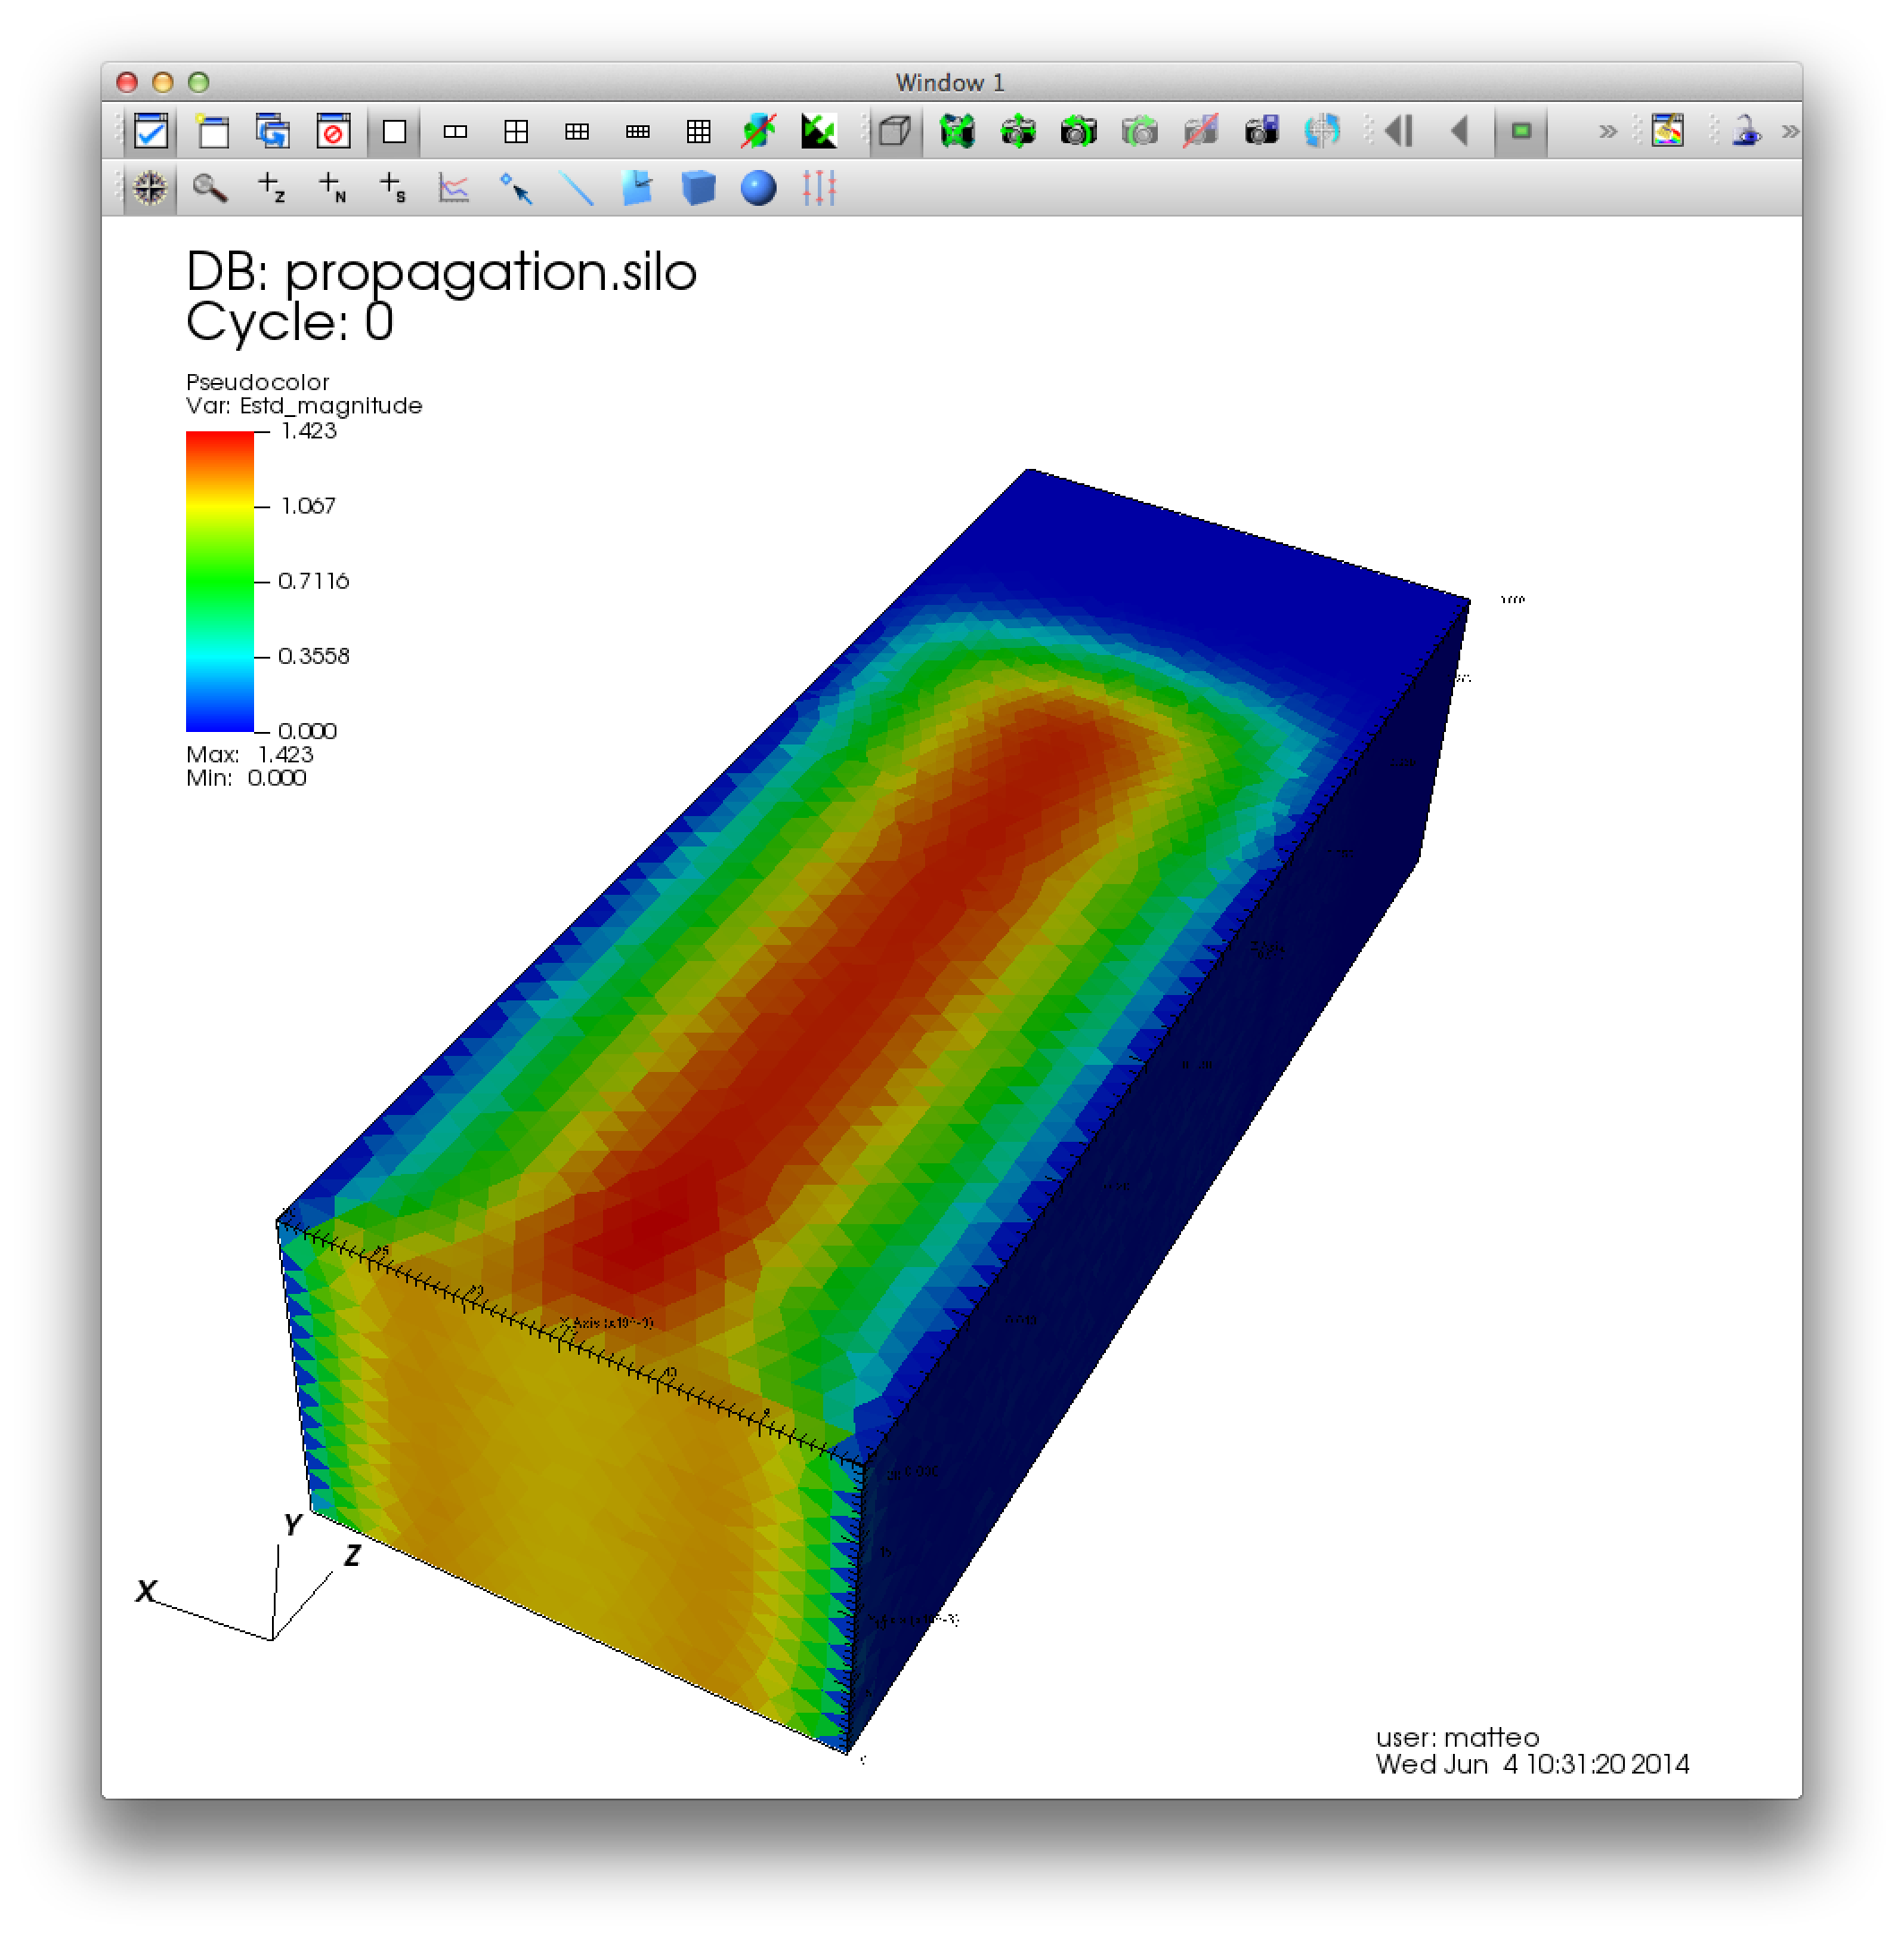
\includegraphics[width=\textwidth]{img/wg_prop.png}
%    \end{minipage}
%}

%\headerbox{Codice di simulazione}{name=simulator,column=0,row=3,span=2,below=radiators}{
%    È stato realizzato un codice di simulazione che implementa l'intera parte numerica della metodologia proposta. Il software è un tool generico per la DGA, espandibile a problemi diversi dalla propagazione elettromagnetica. I moduli attualmente implementati sono:
%    \begin{itemize}
%        \compresslist
%    \item Geometria: supporto efficiente a mesh tetraedriche di grosse dimensioni (50MB/1Melem) e operazioni tipicamente $O(1)$, solo alcune $O(log n)$
%        \item Elettrostatica: modulo per la risoluzione di semplici problemi di test
%        \item Magnetostatica: modulo per la risoluzione di semplici problemi di test
%        \item Propagazione: condizioni di ammettenza, condizioni di porta, formulazione complementare, materiali PML, antenne equivalenti
%        \item Solutori: il software consente la selezione a tempo di esecuzione di diversi risolutori, sia iterativi che diretti
%        \item Postprocessing: supporto alla visualizzazione tramite VisIt e Gnuplot
%        \item Interfaccia utente testuale interattiva e controllabile attraverso file di configurazione
%    \end{itemize}
%}

%\headerbox{Ringraziamenti}{name=future,column=2,row=3,below=radiators}{
%    
\includegraphics[width=0.48\textwidth]{img/emilab.png}%
%    
\includegraphics[width=0.48\textwidth]{img/emcy_logo.pdf}%
%}

%\headerbox{Riferimenti}{name=refack,column=0,row=4,span=3,below=simulator}{

%\begingroup
%\renewcommand{\section}[2]{}

%\begin{thebibliography}{9}
%    \bibitem{DgaAdmit} L. Codecasa, R. Specogna, F. Trevisan, \emph{Discrete geometric formulation of admittance boundary conditions for frequency domain problems over tetrahedral dual grids}, IEEE Transactions on Antennas and Propagation, Vol. 60, No. 8, 2012, pp. 3998-4002
%    \bibitem{SymPosCM} L. Codecasa, R. Specogna, F. Trevisan, \emph{Symmetric positive definite constitutive matrices for discrete Eddy-current problems}, IEEE Transactions on Magnetics, Vol. 42, No. 2, 2007, pp. 510-515
%    \bibitem{Port} M. Cicuttin, S. Chialina, L. Codecasa, R. Specogna, F. Trevisan, \emph{Port boundary conditions for discrete electromagnetic problems in the frequency domain}, Submitted for publication on IEEE Transactions on Magnetics 
%\end{thebibliography}
%
%\endgroup
%
%}


 \end{poster}

\end{document}
